\documentclass[12pt]{article}

\usepackage{polski}
\usepackage[utf8]{inputenc}
\usepackage[T1]{fontenc}
%\usepackage{indentfirst}
\usepackage{amsfonts}
\usepackage{graphicx}
\usepackage{caption}
\usepackage{multirow}
\usepackage{booktabs}
\usepackage{amssymb}
\usepackage[top=2cm, bottom=2cm, left=3cm, right=3cm]{geometry}
\usepackage{mathrsfs}
\usepackage{tikz}
\usepackage{pgfplots}
%\pagestyle{empty}
\usepackage{listings}
\usepackage{titlesec}
\usepackage{hyperref}
\usepackage{graphicx}
\usepackage{subfig}
\usepackage{natbib}
\usepackage{rotating}
\usepackage{float}
\usepackage{pdfpages}
\usepackage{pdflscape}

\title{\textbf{Rekrutacja Scorpio}}
\author{Michał Wieczorek {226284}}
\date{\today}

\begin{document}
\maketitle
\newpage
\section{Wstęp}
Jestem studentem III roku Automatyki i Robotyki na wydziale Elektroniki, interesuję się motoryzacją, elektroniką, robotyką oraz najnowszymi technologiami, np Przemysłem 4.0. Moim pierwszym projektem opartym na mikrokontrolerach był system alarmowy oparty na czujnikach PIR. Brałem udział w warsztatach robotycznych organizowanych przez KoNaR, podjąłem się budowy robota MiniSumo, odkładana w czasie budowa niedawno zakończyła się sukcesem. Od roku uczestniczę w KN EKSA, gdzie grupowo realizuję projekt Systemu Detekcji Wyładowań Atmosferycznych, gdzie do przetwarzania danych i komunikacją z serwerem używamy płytki Nucleo z procesorem STM32. Na co dzień dużo zajmuję się elektroniką i bardzo interesuje mnie Wasz projekt łazika, dlatego chciałbym się stać jednym z jego twórców.

\section{Realizacja}
Podjąłem się realizacji zadania 2. dla elektroników/programistów. Czyli zaprojektowania schematu i płytki PCB zgodnie z wytycznymi. 
\subsection{Schemat układu}
Omawianie schematu pozwolę sobie rozdzielić na kilka części, zgodnie z wytycznymi i własnymi spostrzeżeniami. \\
Sercem prototypu płytki jest 100 nóżkowy procesor $STM32F107VC$. Wybrałem go z powodu możliwości obsługi systemu wymiany danych CAN oraz ETHERNET'u.
\subsubsection{Podstawowe rzeczy}
Przyjąłem że układ będzie zasilany wartością 12V. Oczywiście wartość tą można zmienić, jednak maksymalna wartość napięcia wejściowego nie powinna przekraczać 15V. Nie dodałem żadnego zabezpieczenia elektronicznego przed odwrotną polaryzacją, zastąpiłem je zabezpieczeniem mechanicznym - gniazdo zasilania jack. Dodałem zieloną diodę zasilania, oraz przycisk do resetu układu. 
\begin{figure}[H]
\begin{center}
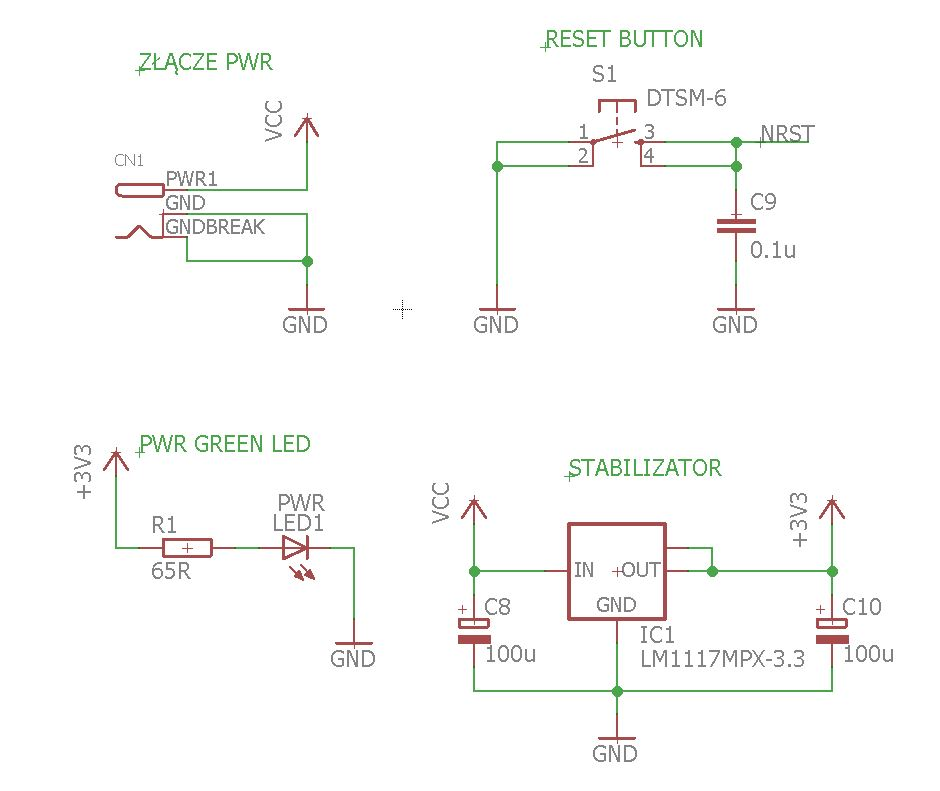
\includegraphics[width=1\textwidth]{figures/schemat1.jpg}
\end{center}
\end{figure}
\subsubsection{Zasilanie mikroprocesora}
W kwestii zasilania, elementy filtrujące dodane zostały w taki sposób, aby układ pracował prawidłowo, stąd odpowiednia ilość kondensatorów przy nóżkach zasilających mikrokontroler.
\begin{figure}[H]
\begin{center}
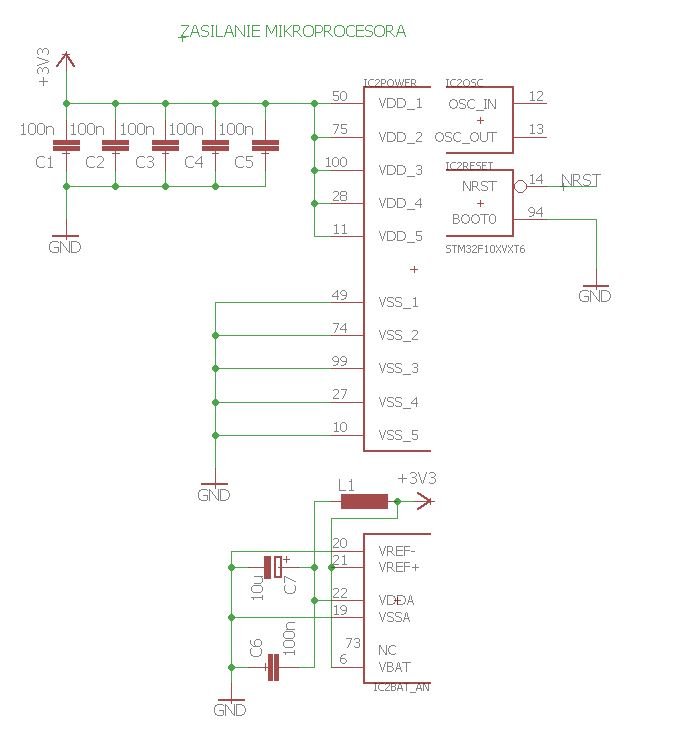
\includegraphics[width=1\textwidth]{figures/schemat2.jpg}
\end{center}
\end{figure}
\subsubsection{IMU}
Zdecydowałem się na położenie układu $LSM9DS1$ bezpośrednio na płytce. Uważam, że niewątpliwą przewagą takiego rozwiązania jest stabilność układu i lepsza dokładność wskazań niż przy zastosowaniu gotowej płytki z modułem do wlutowania, która może nie być wystarczająco sztywna i zakłamywać wskazania. Jak widać na schemacie czujnik posiada możliwość zmiany adresu akcelerometru/żyroskopu oraz magnetometru. (ustawiając odpowiednio zworkę możemy łatwo wyłączyć z działania któryś z modułów. Moduł podłączony jest do mikroprocesora za pośrednictwem magistrali I2C. 
\begin{figure}[H]
\begin{center}
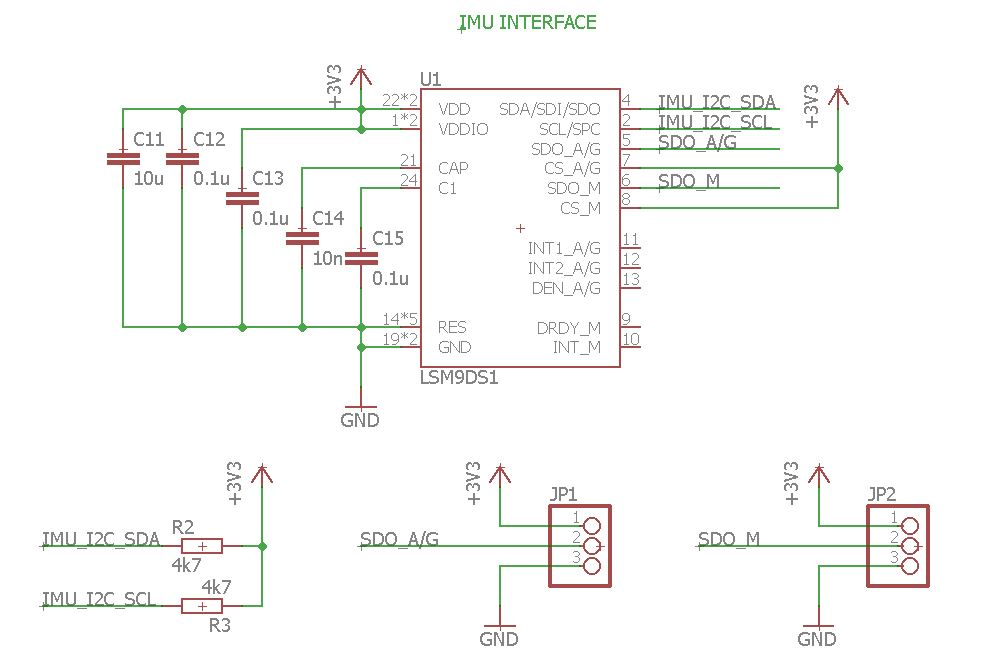
\includegraphics[width=1\textwidth]{figures/schemat3.jpg}
\end{center}
\end{figure}
\subsubsection{CAN}
Co do tego interfejsu, na wyjściu zastosowałem gniazdo RS232. Zworką możemy przełączyć tryb pracy układu.
\begin{figure}[H]
\begin{center}
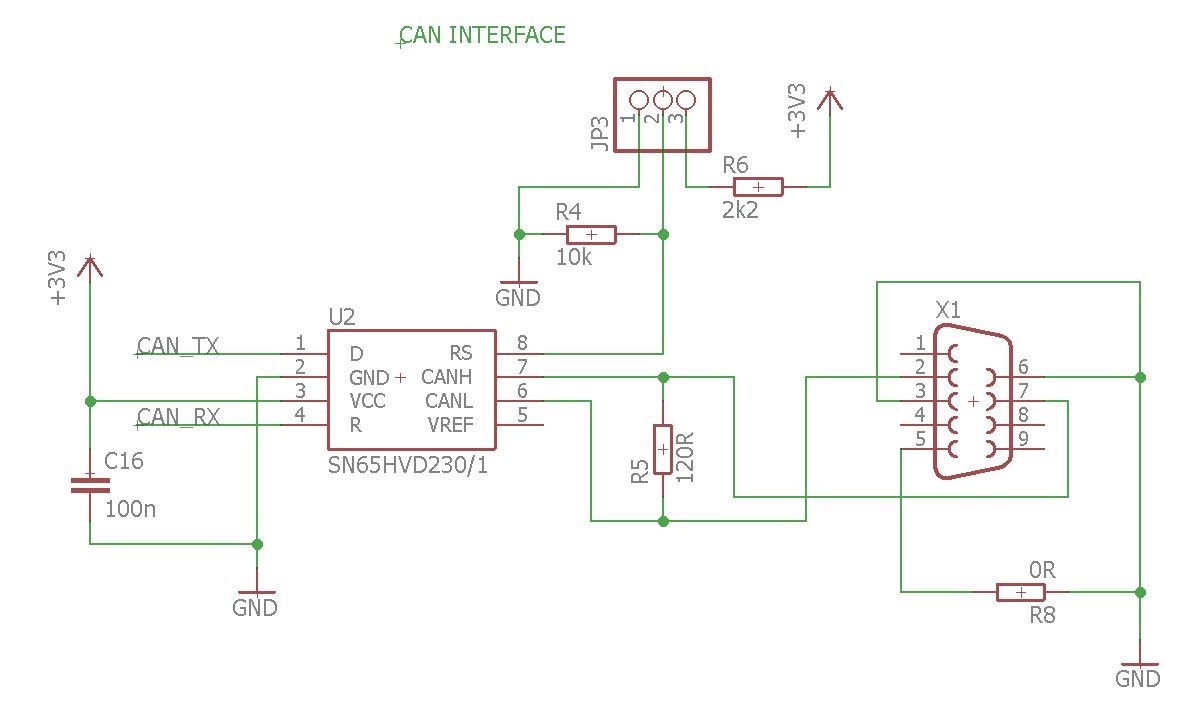
\includegraphics[width=1\textwidth]{figures/schemat4.jpg}
\end{center}
\end{figure}
\subsubsection{Enkoder Absolutny}
Sporo czasu zajęło mi wybranie odpowiedniego interfejsu, na początku chciałem podłączyć enkoder na przerwania, jednak ostatecznie zdecydowałem się na połączenie po SPI. Zaletą takiego rozwiązania jest możliwość podłączenia kilku enkoderów do tej samej linii danych. Gniazdo jakie wyprowadziłem to 6-pinowy goldpin ustawiony pod kątem prostym, pasuje on do enkoderów absolutnych marki $Bourns$, model:$EMS22A$, który został zaprojektowany dla zasilania 3.3V, ale będzie pracował prawidłowo również z innymi enkoderami z możliwością obsługi SPI.
\begin{figure}[H]
\begin{center}
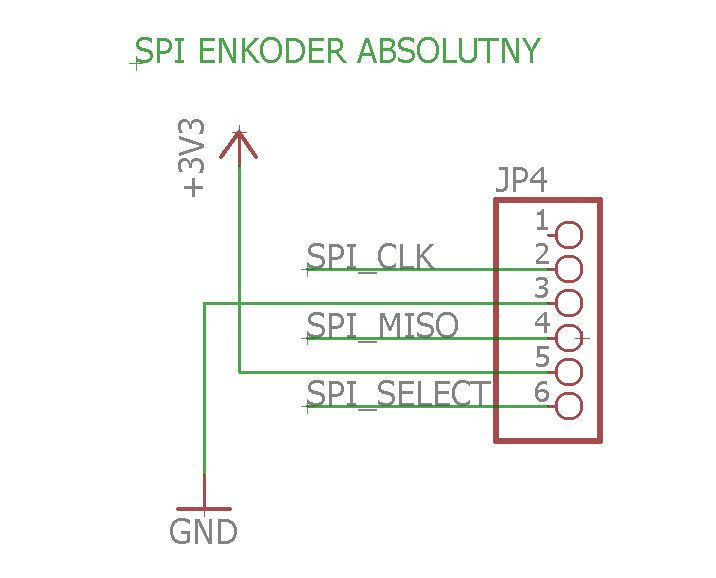
\includegraphics[width=0.5\textwidth]{figures/schemat5.jpg}
\end{center}
\end{figure}
\begin{figure}[H]
\begin{center}
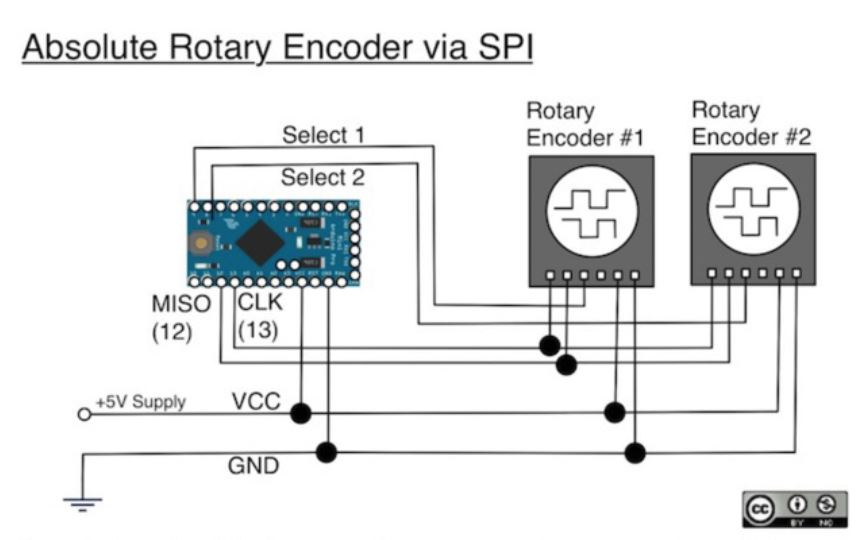
\includegraphics[width=0.8\textwidth]{figures/SPI.jpg}
\end{center}
\end{figure}
\newpage
\subsubsection{Ethernet}
Ten moduł jest najbardziej rozbudowany. Do budowy schematu użyłem układu $DP83848$, wzorowałem się natomiast na gotowym module $ZL3ETH$. Układ posiada oddzielną filtrację zasilania, kwarc taktujący zegarem $25MHz$, który można zmienić w zależności od typu używanej transmisji. Na wyjściu układu znajduje się gniazdo RJ-45 z dwoma diodami stanu, które pokazują wysyłanie/odbieranie danych.
\begin{figure}[H]
\begin{center}
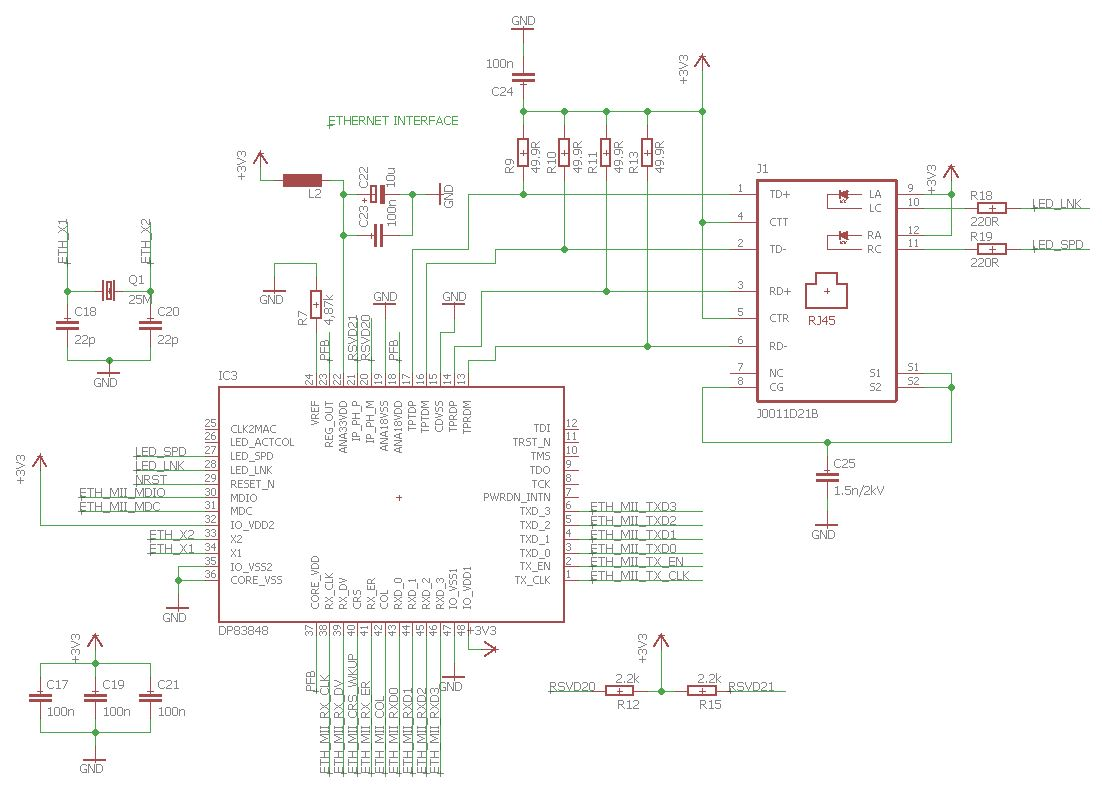
\includegraphics[width=1\textwidth]{figures/schemat6.jpg}
\end{center}
\end{figure}
\subsubsection{Fototranzystor, dioda IR, dioda LED, gniazdo programatora}
Fototranzystor podłączyłem do wejścia ADC1 mikroprocesora, próbkującego sygnał analogowy. Dioda IR podłączona pod gniazdo z obsługą PWM. Tak samo również zwykła dioda LED stanu podłączona pod generator PWM. Nie wiem czy dobrze zrozumiałem zadanie, ale wszystkie 3 elementy usytuowane są w jednym miejscu na płytce. Diodę IR można więc ustawić nad fototranzystorem, tranzystor jako sprzężenie zwrotne będzie generował sygnał PWM na diodzie LED. Więc teoretycznie sygnał PWM na diodzie LED powinien odpowiadać temu wygenerowanemu na diodzie IR.\\
Gniazdo programatora jest dodatkiem ode mnie. Stwierdziłem iż dodanie zwykłego goldpinu mogłoby być dość uciążliwe przy ciągłym wpinaniu i wypinaniu wtyczki, dlatego zastosowałem gniazdo miniUSB. 
\begin{figure}[H]
\begin{center}
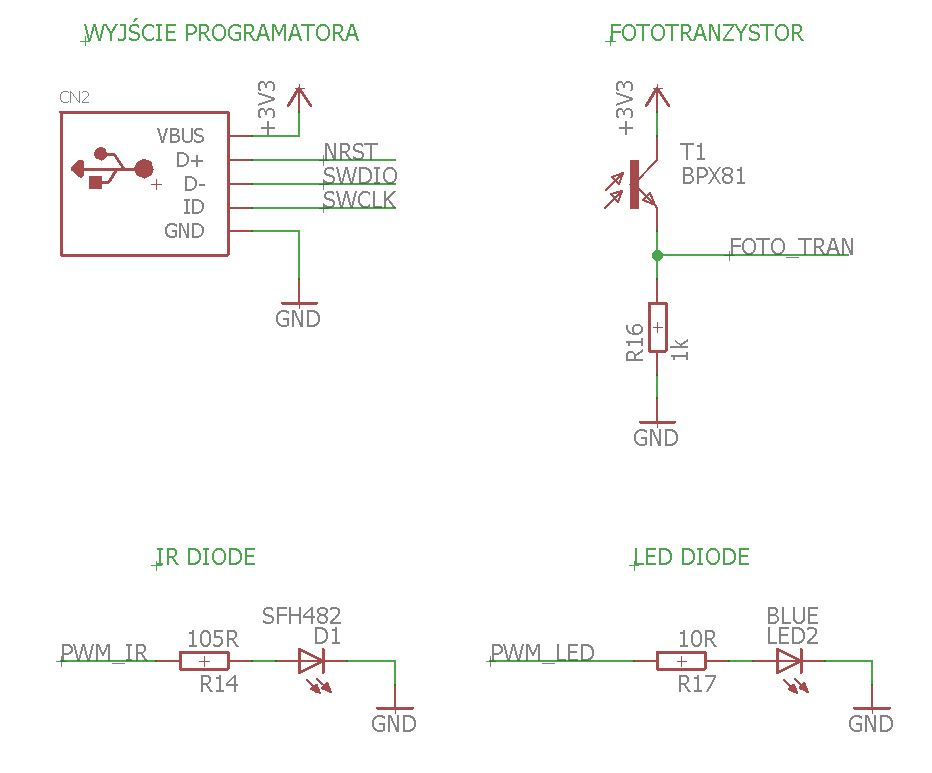
\includegraphics[width=0.8\textwidth]{figures/schemat7.jpg}
\end{center}
\end{figure}
\subsubsection{Przyciski i diody LED}
Ponieważ przy mikroprocesorze zostało sporo wolnych pinów zdecydowałem o umieszczeniu dodatkowych 3 przycisków oraz 3 diód LED w kolorach (zielonym, żółtym, czerwonym). Mogą się one przydać np. do pokazywania różnych stanów płytki, usterek czy awarii, natomiast przyciski do zmieniania ustawień.
\begin{figure}[H]
\begin{center}
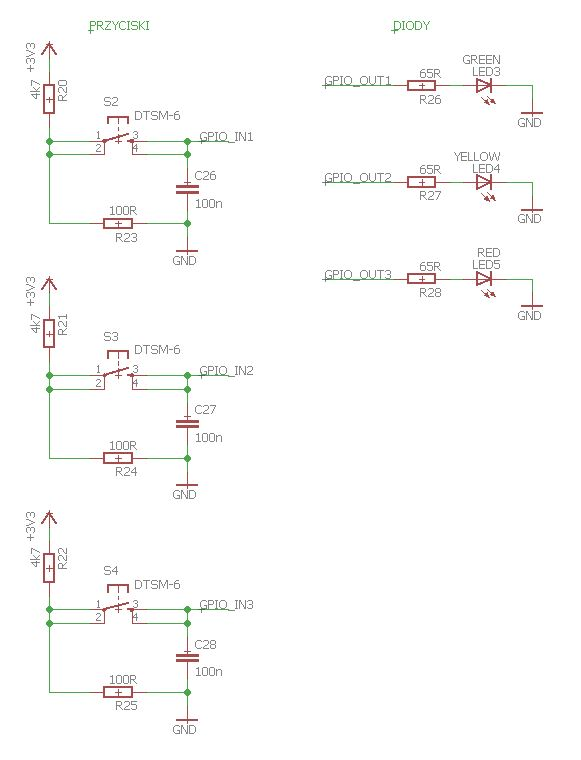
\includegraphics[width=0.8\textwidth]{figures/schemat8.jpg}
\end{center}
\end{figure}
\subsubsection{Podłączenie wyprowadzeń procesora}
\begin{figure}[H]
\begin{center}
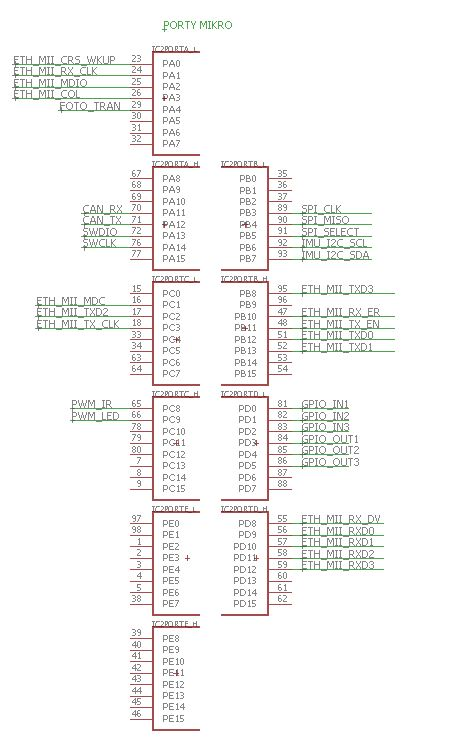
\includegraphics[width=0.8\textwidth]{figures/schemat9.jpg}
\end{center}
\end{figure}
\subsection{Projekt PCB}
Zaprojektowana przeze mnie płytka jest dwuwarstwowa. W projekcie użyłem opcji Autoroutera, który poprowadził dla mnie ścieżki w 80 procentach, resztę naniosłem ręcznie. Wersja studencka programu, której używałem,  nie pozwalała na zwiększenie wymiarów obszaru roboczego powyżej 10 cm x 8 cm. Ścieżki zasilania są pogrubione, elementy filtrujące starałem się umieszczać jak najbliżej układów scalonych.
\begin{figure}[H]
\begin{center}
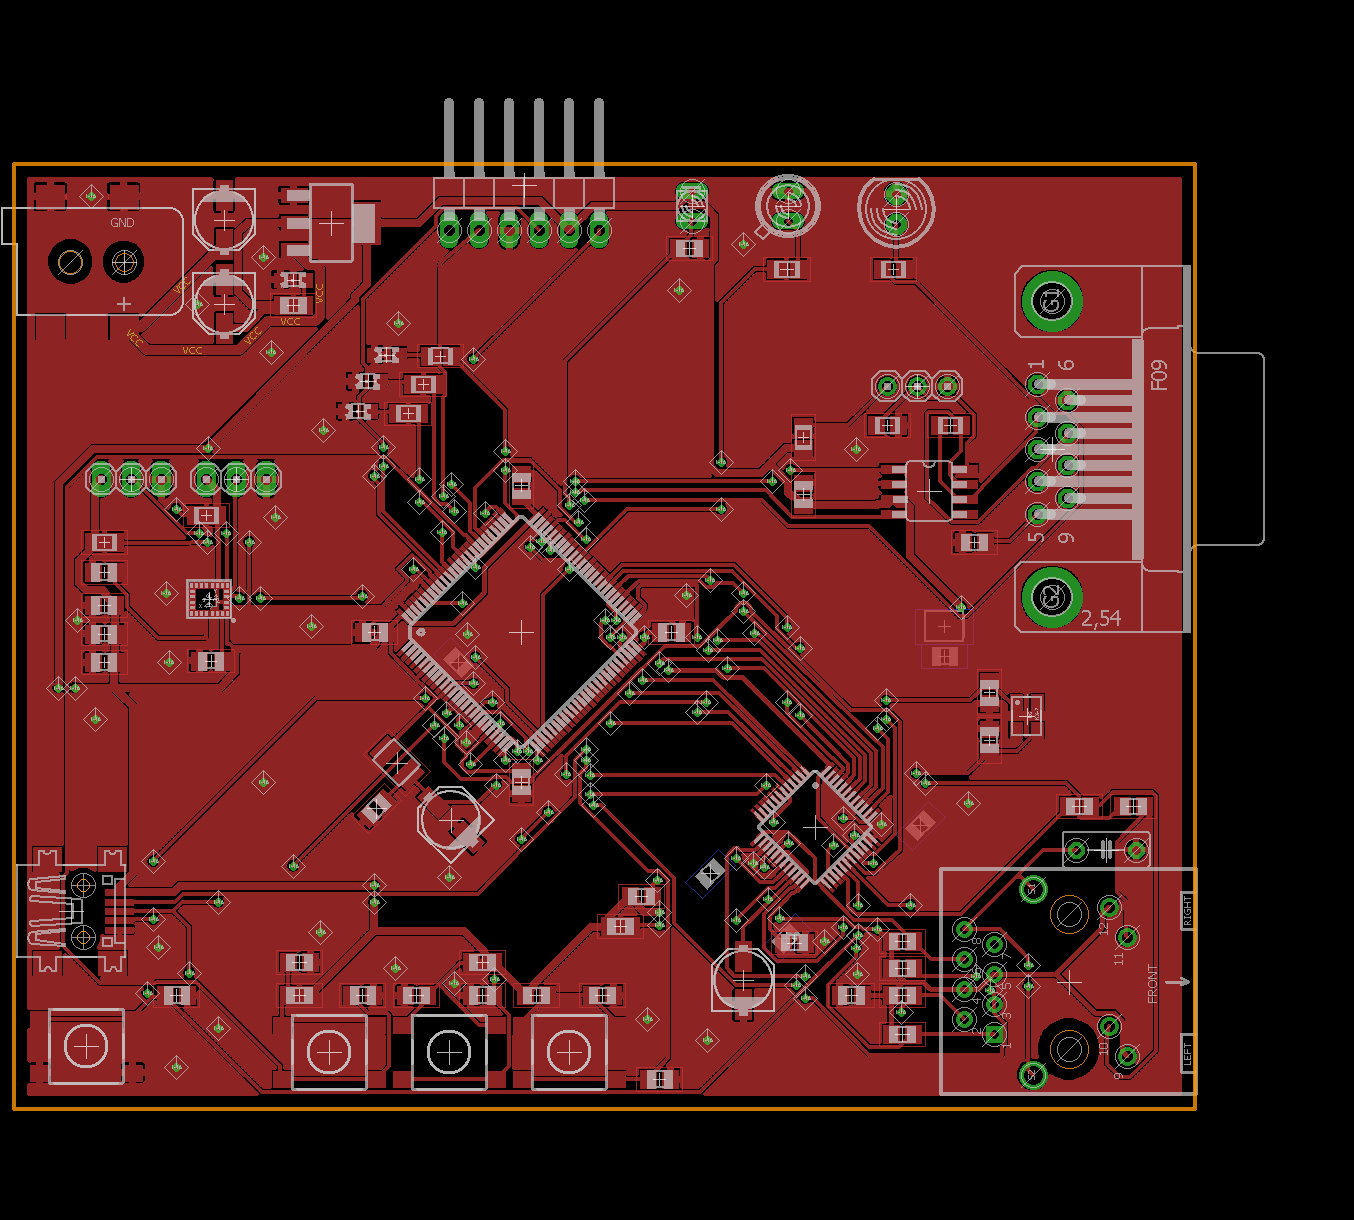
\includegraphics[width=1\textwidth]{figures/top.png}
\caption{Górna warstwa}
\end{center}
\end{figure}

\begin{figure}[H]
\begin{center}
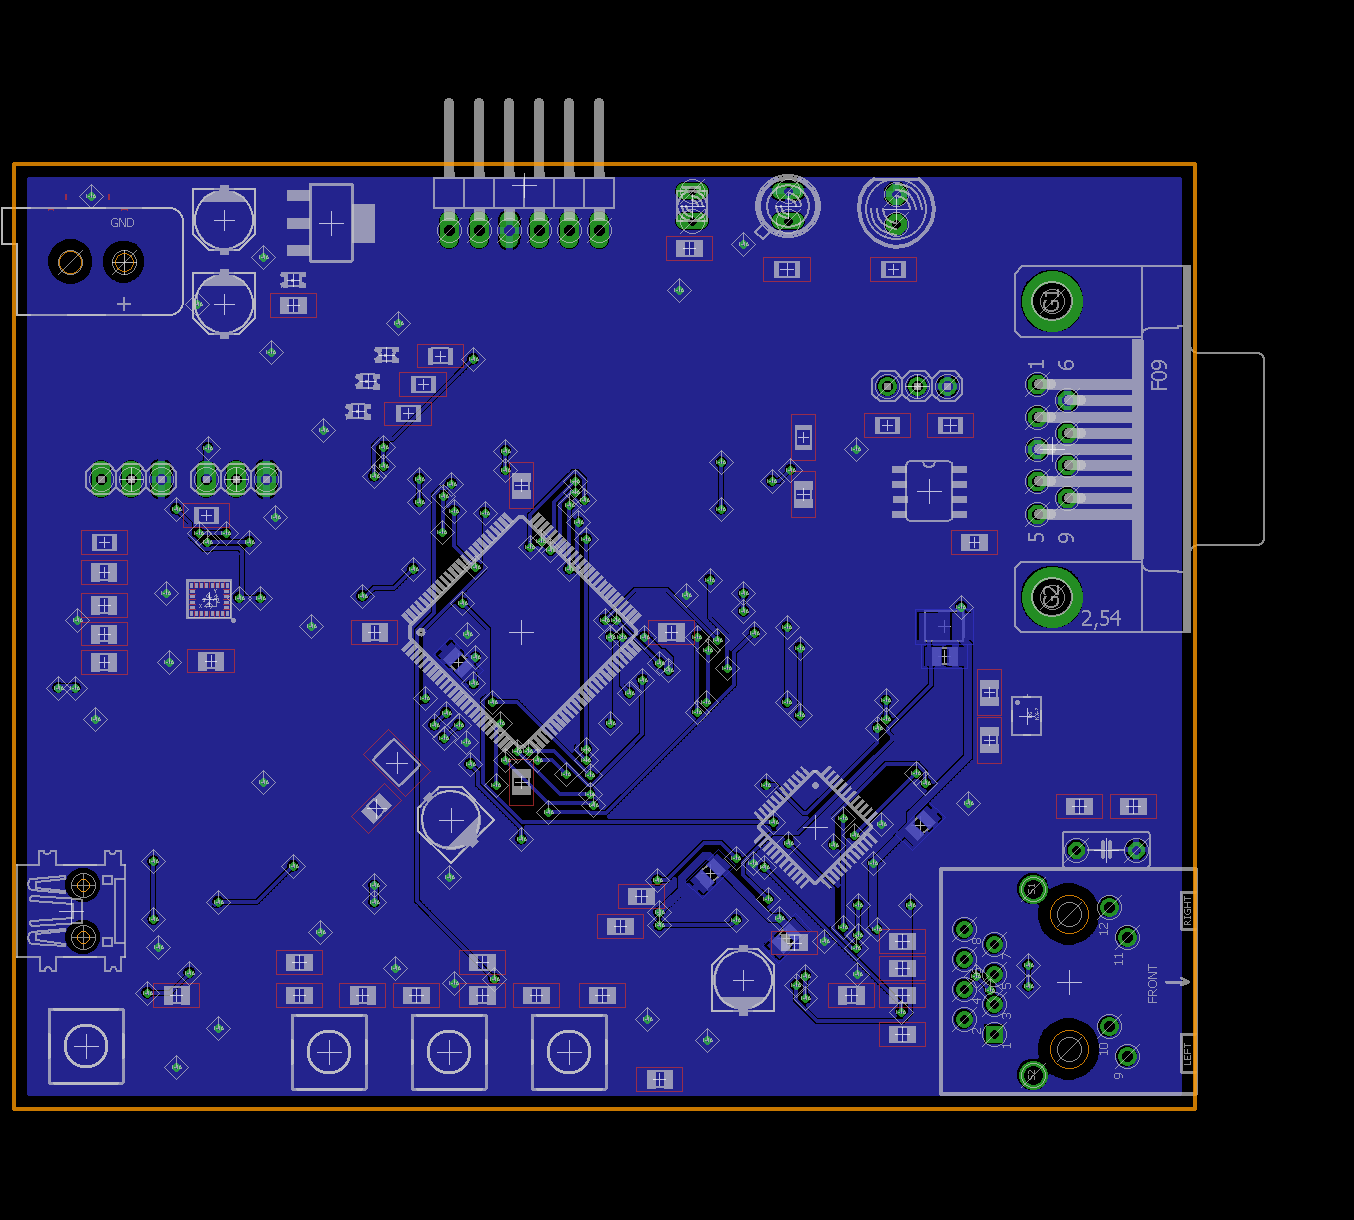
\includegraphics[width=1\textwidth]{figures/bottom.png}
\caption{Dolna warstwa}
\end{center}
\end{figure}

\begin{figure}[H]
\begin{center}
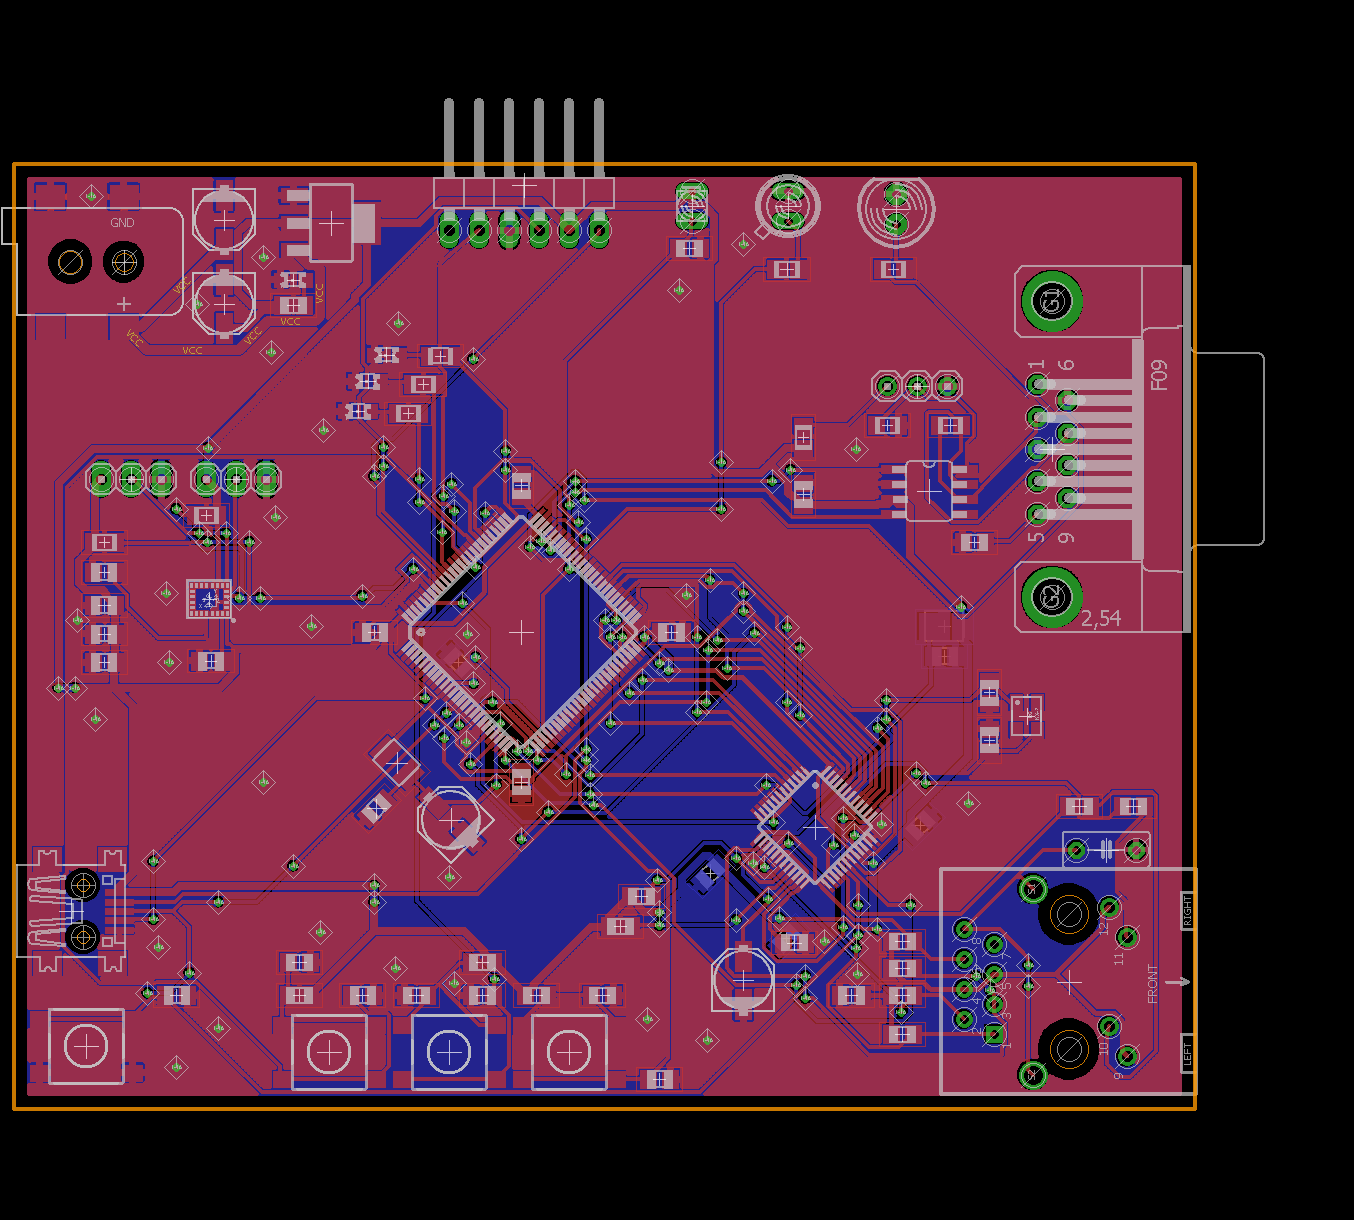
\includegraphics[width=1\textwidth]{figures/all.png}
\caption{Połączenie warstw}
\end{center}
\end{figure}
Poniżej wstawiam zdjęcia prototypu w 3D, jakby to wygłądało wizualnie po złożeniu, na spodzie znajduje się tylko kilka elementów, które przeszkadzały na górnej warstwie.
\begin{figure}[H]
\begin{center}
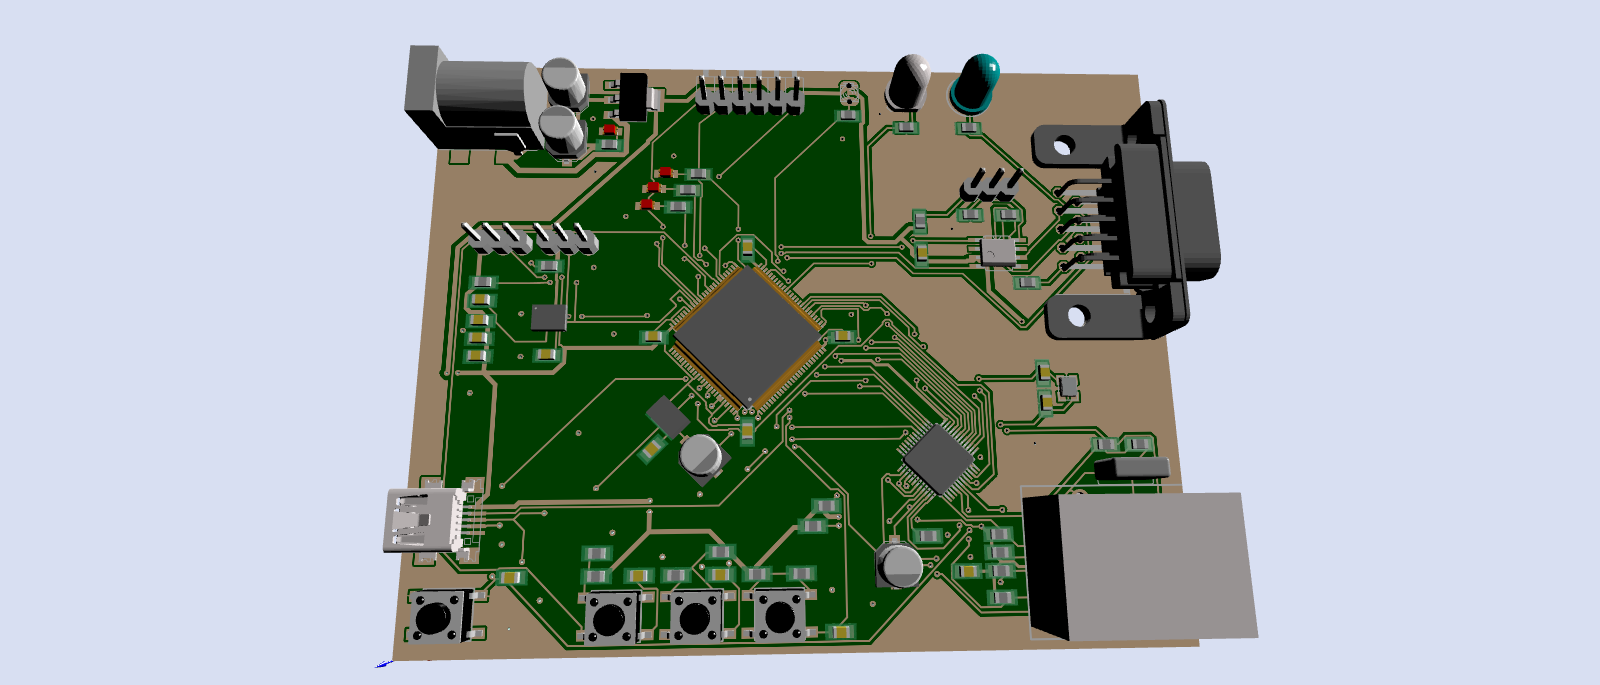
\includegraphics[width=1\textwidth]{figures/pcb1.png}
\end{center}
\end{figure}

\begin{figure}[H]
\begin{center}
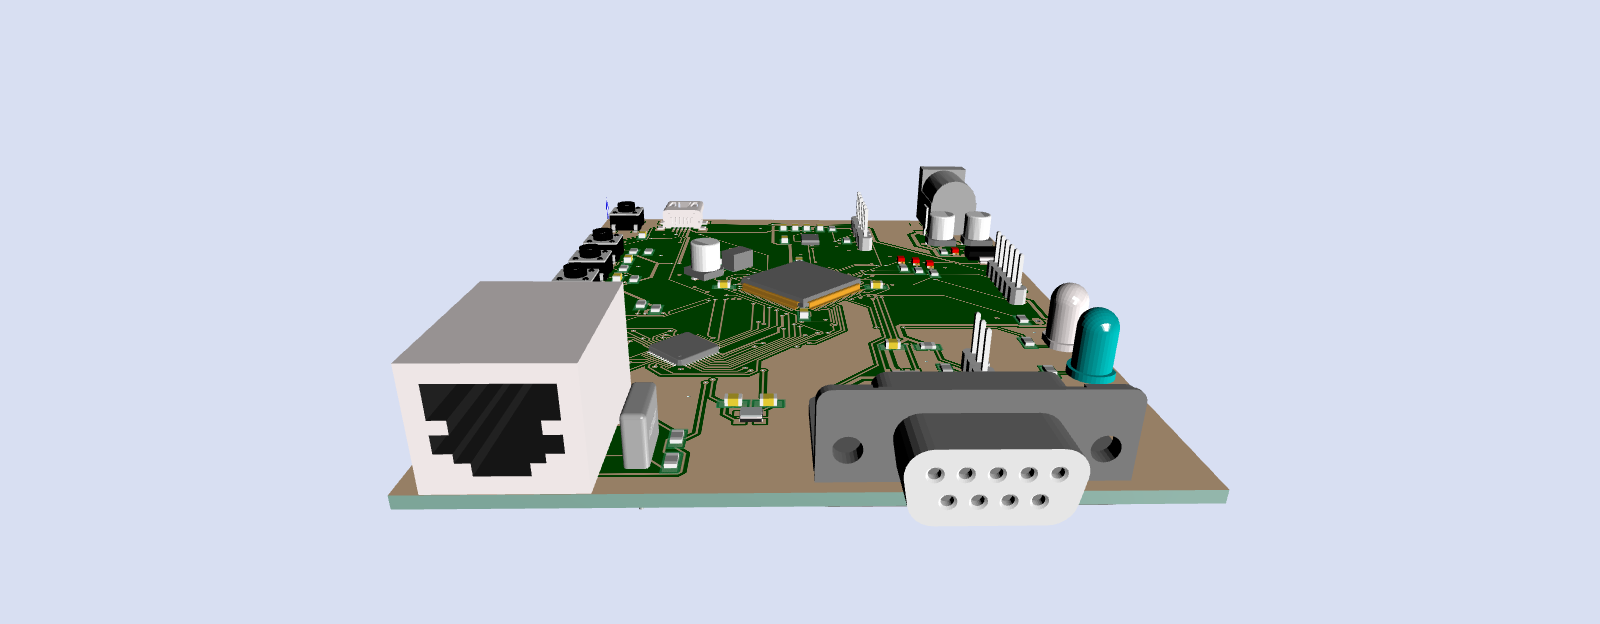
\includegraphics[width=1\textwidth]{figures/pcb2.png}
\end{center}
\end{figure}

\begin{figure}[H]
\begin{center}
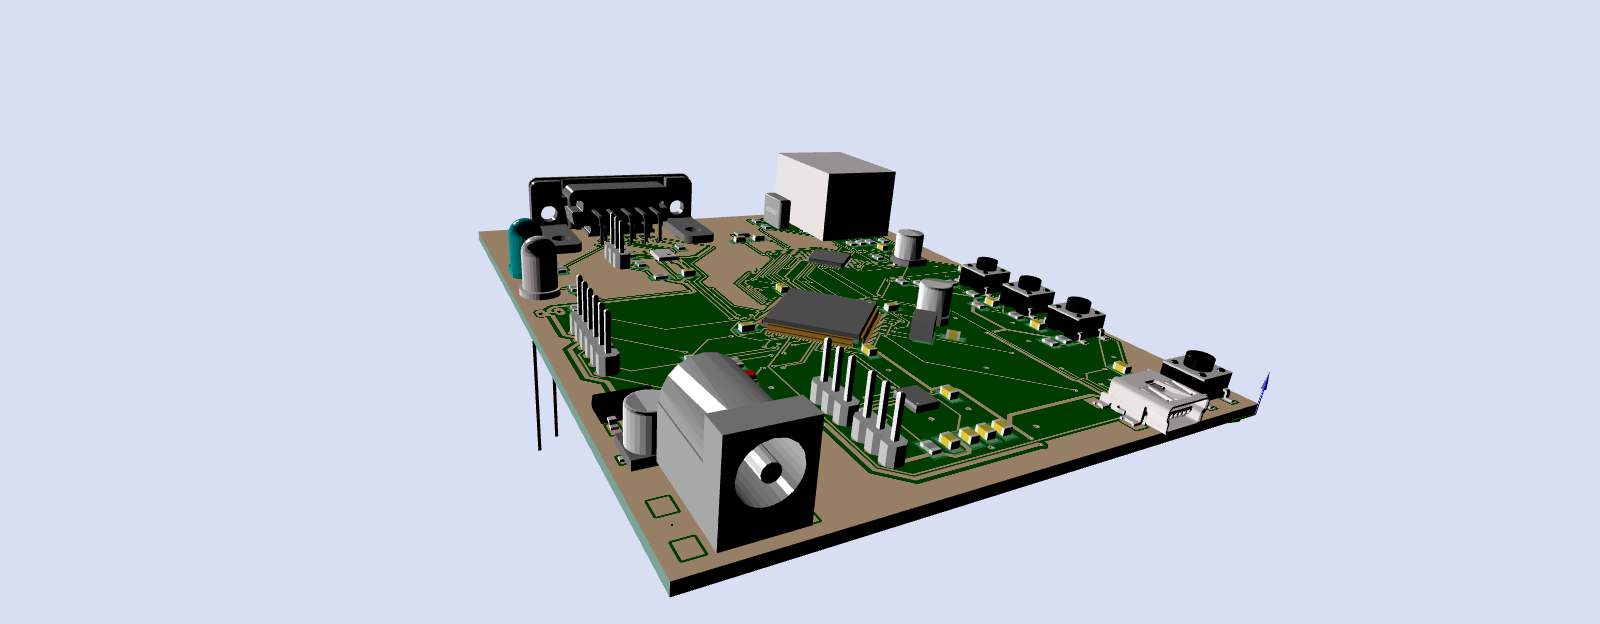
\includegraphics[width=1\textwidth]{figures/pcb3.png}
\end{center}
\end{figure}

\subsection{Programowanie i prototyp}
Poniższy rysunek przedstawia konfigurację portów w programie Cube MX, do programowania użyłbym biblioteki HAL.
\begin{figure}[H]
\begin{center}
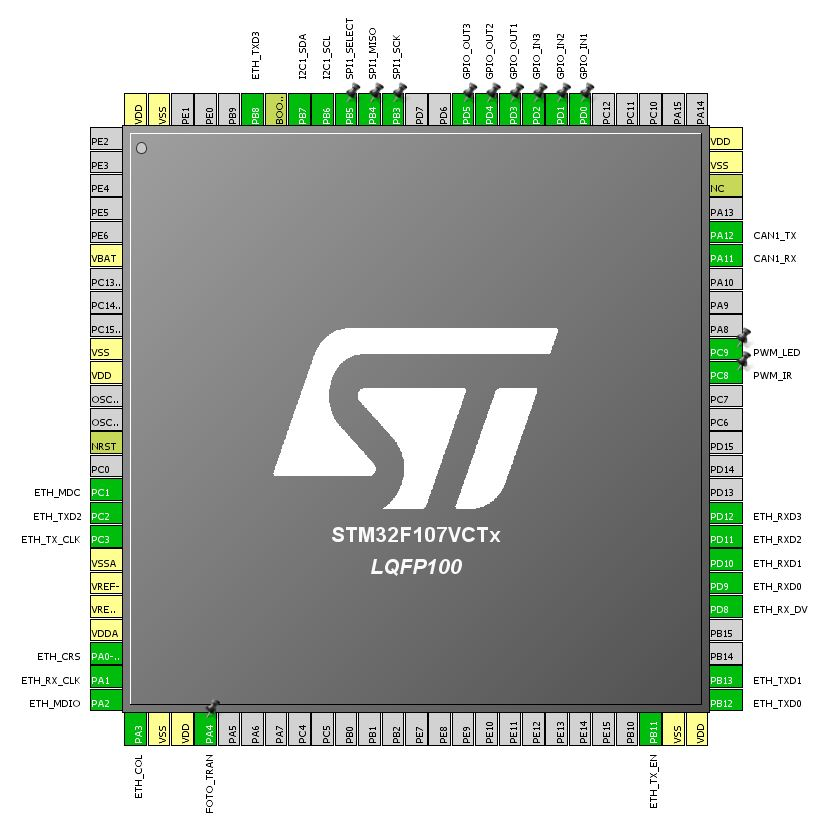
\includegraphics[width=1\textwidth]{figures/cube.jpg}
\end{center}
\end{figure}

\section{Podsumowanie}
Do sprawozdania załączam archiwum, w którym znajdują się elementy projektu - schemat połączeń i projekt płytki w formacie EAGLE'a, a także biblioteki których używałem przy projektowaniu. Z racji braku czasu prototyp oraz programowanie płytki są kwestią niedokończoną. W razie potrzeby kontaktu ze mną na temat projektu proszę o kontakt pod poniższy adres e-mail: michal126@hotmail.com.

\end{document}

